In questo capitolo è descritta la metodologia del sistema di correzione.\\
Nella \autoref{sec:met_introduzione} vengono descritti gli obiettivi del processo di correzione e le criticità che lo contraddistinguono.
Nella \autoref{sec:met_panoramica} è presente una panoramica generale del processo di correzione, e sono le fasi e le componenti del sistema. Nella \autoref{eq:met_BERT} è descritto il funzionamento del BERT MLM, che sta alla base del processo di correzione. Nelle sottosezioni \ref{sec:met_tok_correct} e \ref{sec:met_mod_split} è descritto il funzionamento dei moduli che stanno alla base del sistema di correzione.


\section{Introduzione}
\label{sec:met_introduzione}
L'optical character recognition, o OCR, è una tecnologia tramite la quale è possibile estrarre e digitalizzare del testo da un'immagine. Più precisamente, per digitalizzare si intende ottenere del testo in una una codifica leggibile da una macchina, come ad esempio ASCII o Unicode.

\begin{figure}[H]
\centering
{
\begin{minipage}{0.4\textwidth}
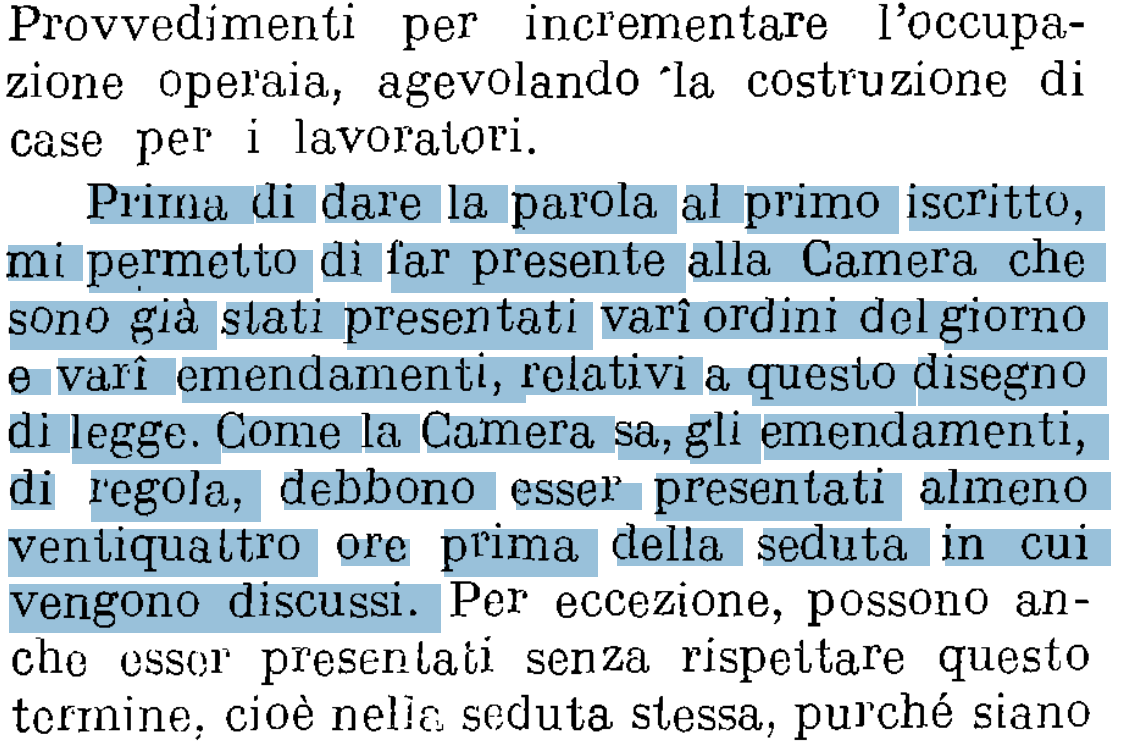
\includegraphics[width=\textwidth]{immagini/metodologia/ocr_ex.png}
\end{minipage} \hfill
\begin{minipage}{0.06\textwidth}
\Large$\rightarrow$
\end{minipage}
\begin{minipage}{0.5\textwidth}
\footnotesize	
Prima. di dare la parola al primo iscritto, \\
mi permetto di far presente alla Camera che \\
sono già stati presentati vari ordini del giorno \\
e var.1 emendamenti, relativi a questo disegno \\
di legge. Come la Camera sa, gli emendamenti, \\
di regola, debbono esser presentati alrneno \\
ventiquattro ore prima della seduta in cui \\
vengono discussi.
\end{minipage}
\caption{Esempio di testo estratto tramite OCR}
\label{fig:met_ocr_esempio}
}
\end{figure}

L'uso di sistemi OCR è particolarmente vantaggioso per l'archiviazione dei documenti. Infatti, l'estrazione del testo rende possibile eseguire sui documenti operazioni di ricerca e di reperimento informazioni. Si pensi a un'operazione basilare come la ricerca di tutti i documenti che contengono una determinata parola: un task dispendioso e manuale che è quasi istantaneo se si ha a disposizione il testo digitalizzato.
\paragraph{Errori}
I sistemi OCR presentano però alcuni problemi che possono influenzare negativamente le performance nel reperimento di informazioni \cite{impatto_ocr_1}\cite{impatto_ocr_2}. Si veda, ad esempio, il testo estratto in \autoref{fig:met_ocr_esempio}: seppur la maggior parte delle parole sono state riconosciute correttamente, è possibile notare alcuni errori. 
Generalmente la presenza di tali errori è dovuta a piccole imprecisioni nell'immagine iniziale: si pensi ad esempio un granello di polvere che può essere scambiato per un punto, o ad una \textit{"n"} battuta male che viene scambiata per la sequenza \textit{"ii"}.
Si possono distinguere le seguenti categorie di errore:
\begin{itemize}
\item \textbf{Errore di token}. Si ha un errore di token quando aggiunte, rimozioni o sostituzioni di caratteri occorrono all'interno di una parola senza però dividerla o eliminarla. Questo tipo di errore si divide in due ulteriori sottocategorie:
	\begin{itemize}
	\item Non-word error (NW), quando la parola risultante non è presente in un dato vocabolario.
	\item Real-word error (RW), quando la parola risultante è presente in un dato vocabolario.
	\end{itemize}
	
\item \textbf{Errore di segmentazione}. Si ha un errore di segmentazione quando aggiunte, rimozioni o sostituzioni di caratteri occorrono in maniera tale da dividere o unire parole. Sono considerati errori di segmentazione anche aggiunte di caratteri e segni di punteggiatura spuri all'interno del testo. Sono distinte le seguenti sottocategorie di errori di segmentazione:
	\begin{itemize}
	\item Spezzettamento con spazi (SP), quando i caratteri di una parola o più parole adiacenti sono intervallati da spaziature.
	\item Divisione con punteggiatura (DP), quando un segno di punteggiatura divide in due una parola.
	\item Punteggiatura spuria (PS), quando un segno di punteggiatura viene aggiunto fra una parola e l'altra.
	\end{itemize}
\end{itemize}

In \autoref{tab:met_esempio_errori} sono riportati alcuni esempi di errori.

\begin{table}[H]
\centering
\begin{tabular}{cccc}
\textbf{Originale} & \textbf{OCR} & \textbf{Tipo} & \textbf{Errore} \\ \hline
dell'impresa & dell’iinpresa 	& NW & Sostituzione di "m" con "in" \\
interessano & iateressano 		& NW & Sostituzione di "n" con "a" \\
questo modo & questo nodo 		& RW & Sostituzione di "m" con "n" \\
l'ingordizia & I’ingordizia 	& RW & Sostituzione di "l" con "I" \\
produttrice & pro d u t t rice 	& SP & Parola spezzettata da spazi \\
azionisti & azi:misti 			& DP & Sostituzione con divisione della parola \\
vicinanze  del & vicinanze .del & PS & Introduzione di punteggiatura\\

\end{tabular}
\caption{Esempi di errori}
\label{tab:met_esempio_errori}
\end{table}

Se, come già detto, gli errori derivano spesso da piccoli difetti nell'immagine di partenza, è lecito aspettarsi una maggior quantità di errori da documenti di più deteriorati, come archivi storici. Per lo stesso motivo l'intensità degli errori può variare a seconda delle specifiche condizioni delle specifiche parti del documento.

\paragraph{Post-processing}
Una strategia spesso adottata per minimizzare il numero di errori è l'aggiunta di
una fase di post elaborazione (OCR post-processing) in seguito all'acquisizione
dei documenti tramite OCR. Lo scopo della fase di OCR post-processing è quello di correggere gli errori introdotti durante l'estrazione del testo dalle immagini. Una delle difficoltà in questa fase sta nel non introdurre nuovi errori nel testo. Si pensi ai seguenti casi:
\begin{itemize}
\item Il sistema prova a correggere una parola che non contiene errori. In questo caso, qualsiasi correzione risulterà in un nuovo errore. Una delle maggiori criticità nello sviluppare il sistema di correzione, infatti, sta nell'identificare correttamente gli errori all'interno del testo.
\item Il sistema identifica correttamente un errore, ma propone una correzione sbagliata. Si pensi al seguente esempio: la parola \textit{"amati"} viene riconosciuta come \textit{"amolfi"}. Il sistema potrebbe correggere con \textit{"amati"}, introducendo un errore.
\end{itemize}

\ \\
La metodologia di correzione sviluppata è modellata come una pipeline che si compone di una serie di moduli ripetibili in sequenza. Ogni modulo è una funzione che si occupa di individuare e correggere una specifica categoria di errore.\\
La metodologia sviluppata si propone di correggere i real-word error (RW) e gli errori di spezzettamento con spazi (SP).

\section{Architettura del sistema}
\label{sec:met_processo}

\subsection{Panoramica Generale}
\label{sec:met_panoramica}
Il sistema di correzione è articolato come una pipeline composta da uno o più moduli 	concatenati. Un modulo è una funzione il cui scopo è correggere una specifica tipologia di errori all'interno di una frase. Un modulo può essere formalmente definito come segue:
\begin{equation}
M: F \mapsto F\prime
\end{equation}
dove $F$ e $F\prime$ sono rispettivamente la frase originale e quella con delle correzioni apportate. \\
Sono stati definiti i seguenti moduli:
\begin{itemize}
\item \textbf{Modulo di correzione Token} ($M_{TK}$): individua e corregge tutti gli errori di tipo RW. \E\ discusso in dettaglio nella \autoref{sec:met_tok_correct}.
\item \textbf{Modulo di correzione Split} ($M_{SP}$): individua e corregge tutti gli errori di tipo SP. \E\ discusso in dettaglio nella \autoref{sec:met_mod_split}.
\end{itemize}

\begin{figure}[H]
\centering
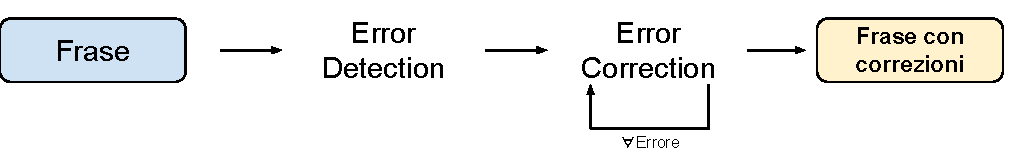
\includegraphics[width=\textwidth]{immagini/metodologia/modulo}
\caption{Schema del funzionamento di un modulo}
\label{fig:met_modulo}
\end{figure}

Come si può vedere in \autoref{fig:met_modulo}, il funzionamento di un modulo si compone delle fasi Error Detection (che da qui in poi sarà abbreviata con ED) ed Error Correction (che da qui in poi sarà abbreviata con EC). Durante la fase di ED vengono individuati gli errori presenti all'interno dalla frase da correggere: dato che moduli differenti correggono tipologie di errore differenti, ogni modulo applica una diversa strategia per individuare gli errori. Nella fase di EC vengono effettuate le correzioni degli errori individuati nella fase precedente.

\paragraph{Esempio} Si supponga di voler applicare alla seguente frase il modulo di correzione token:
\begin{center}
\textit{"\dashuline{Q o a l c h n} Papa \ul{nort} è compreso in questa comunità \ul{d1} morti \ul{gluriosi}"}
\end{center}
Il modulo di correzione token riconosce e corregge solo gli errori di tipo NW (Non-word error, sottolineati con linea continua), mentre ignora tutti gli errori di altro tipo (sottolineati con linea tratteggiata). L'output del modulo, supponendo di riuscire a correggere tutti gli errori, è il seguente:
\begin{center}
\textit{"\dashuline{Q o a l c h n} Papa non è compreso in questa comunità di morti gloriosi"}
\end{center}
\ \\
Data la definizione di modulo, è possibile definire una pipeline di correzione come una concatenazione di uno o più moduli. Più formalmente, una pipeline di correzione è definita come segue:
\begin{equation}
P: f_1 \circ f_2 \circ ... \circ f_n
\end{equation}
dove ogni $f_i$ è un modulo.
\begin{figure}[H]
\centering
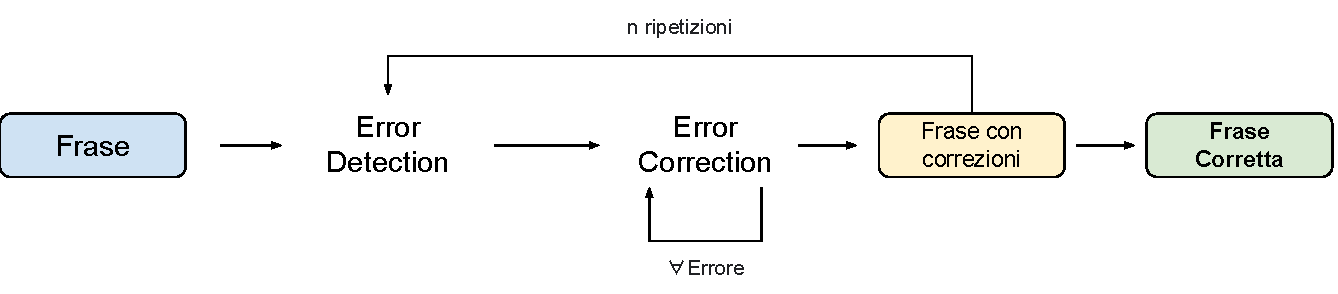
\includegraphics[width=\textwidth]{immagini/metodologia/generale}
\caption{Schema riassuntivo della pipeline di correzione}
\label{fig:met_generale}
\end{figure}

\paragraph{Esempio} Continuando l'esempio precedente, si supponga di concatenare un modulo $M_{SP}$ al precedente modulo $M_{TK}$. Il modulo riceve come input la frase con le correzioni apportate dal modulo precedente, e corregge tutti gli errori di tipo SP presenti nella frase (ovvero quelli con la sottolineatura tratteggiata):
\begin{center}
\textit{"Qualche Papa non è compreso in questa comunità di morti gloriosi"}
\end{center}



\ \\
All'interno della pipeline di correzione possono essere presenti più occorrenze di uno stesso modulo. In frasi con molti errori una sola applicazione di un dato modulo di correzione potrebbe non essere sufficiente per correggere tutti gli errori della propria tipologia. Per ragioni legate al funzionamento del BERT Masked Language Model che verranno meglio chiarite nelle prossime sottosezioni, infatti, ripetere un dato modulo più volte può aumentare tangibilmente le performance di correzione.

\begin{figure}[H]
\centering
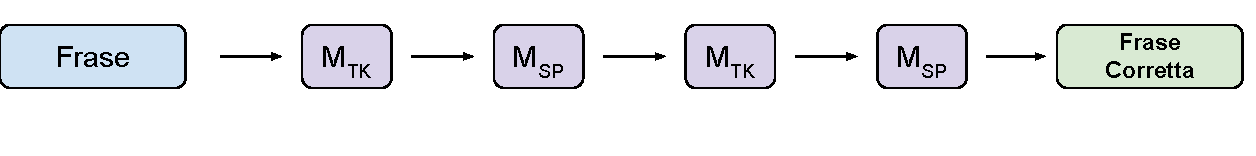
\includegraphics[width=\textwidth]{immagini/metodologia/pipeline_esempio}
\caption{Esempio di una possibile pipeline con più occorrenze di uno stesso modulo}
\label{fig:met_pipeline_esempio}
\end{figure}




\subsection{BERT Masked Language Modeling}
\label{sec:met_BERT_MLM}
La fase di error correction di entrambi i moduli implementati fa uso del BERT Masked Language Modeling (da qui in poi riferito come BERT MLM). Data una qualsiasi sequenza $S = [w_1,...,w_n]$ nella quale ogni $w_i$ è una parola, è possibile mascherare una sola parola $w_i$ con la stringa \textit{[MASK]}. Si ottiene così la sequenza con maschera $S\prime = [w_1,...,\text{[MASK]},...,w_n]$.\\
Dando in input $S\prime$ al modello BERT, esso associa ad ogni parola del proprio lessico la probabilità di corrispondere la parola mascherata. Le prime n parole con la probabilità più alta sono dette candidati.
\E\ quindi formalizzata come segue la funzione del BERT MLM detta "mask-filling":
\begin{equation} \label{eq:met_BERT}
B: S\prime \rightarrow [c_1,...,c_n]
\end{equation}
dove ogni $c_i \in[c_1,...,c_n]$ è un candidato. 

\paragraph{Esempio} Data la frase 
\begin{center}
\textit{"che assistono ragazze in difficoltà, le persone \underline{soie} e abbandonate, gli ammalati e gli anziani."}
\end{center}
la parola \textit{"soie"} sottolineata è stata individuata come errore. \E\ quindi necessario mascherala, per dare la frase in input al modello BERT. La frase diventa dunque:
\begin{center}
\textit{"che assistono ragazze in difficoltà, le persone [MASK] e abbandonate, gli ammalati e gli anziani."}
\end{center}
BERT produce quindi una lista di candidati, di cui sono riportati solo i primi 5:
\begin{itemize}
\item \textit{"sole"} con probabilità 0.42
\item \textit{"anziane"} con probabilità 0.28
\item \textit{"povere"} con probabilità 0.08
\item \textit{"care"} con probabilità 0.03
\item \textit{"disabili"} con probabilità 0.01
\end{itemize}
\ \\
Bisogna sottolineare come la parola originale sia trasparente al modello BERT. Ciò significa che i candidati prodotti dal modello sono del tutto indipendenti dalla parola originale, e sono inferite unicamente dal contesto derivato dal resto della frase.\\




\subsection{Modulo di correzione Token}
\label{sec:met_tok_correct}

\subsubsection{Error Detection}
\label{sec:met_tok_errdet}
Il modulo di correzione token ha lo scopo di individuare e correggere tutti i non-word error (NW).  L'individuazione degli errori è effettuata in modo automatico dopo
una pre-elaborazione (pre-processing) del testo. Il funzionamento di questa
fase può quindi essere suddiviso in due stadi:

\begin{enumerate}
\item \textbf{Pre-elaborazione}: la frase viene tokenizzata, ovvero viene divisa singole parole dette token. Questo stadio è implementato tramite la libreria NLTK\cite{nltk}.
\item \textbf{Identificazione degli errori}: ogni token è analizzato singolarmente per determinare se contenga o meno un errore. Un token è considerato errato se sono vere le seguente condizioni:
	\begin{itemize}
	\item Ha una lunghezza minima di 2 caratteri. Questa condizione è necessaria per evitare di introdurre nuovi errori correggendo inutilmente errori di tipo SP. Ad esempio, sarebbe deleterio provare a correggere le singole lettere di \textit{"Q u a l c h e"}.
	\item Dato un vocabolario di parole corrette, il token considerato non è presente in tale vocabolario. La ricerca nel vocabolario è eseguita in maniera case-insensitive.
	\end{itemize}
Un'eccezione a quest'ultima condizione è data da tutti i token che precedono un apostrofo. Questi token sono considerati corretti se almeno una fra tutte le combinazioni token + vocale è corretta. Si prenda ad esempio il token \textit{"dell"} non presente nel vocabolario, seguito dal token apostrofo. Vengono generate le 5 combinazioni token-vocale \textit{"della"},\textit{"delle"},\textit{"delli"},\textit{"dello"},\textit{"dellu"}. Siccome almeno una di queste è corretta, il token è considerato corretto.
\end{enumerate}

Il processo appena descritto è schematizzato in \autoref{fig:met_tok_errdet}. Tutti gli errori identificati sono poi corretti in sequenza dalla fase di error correction. 

\begin{figure}[H]
\centering
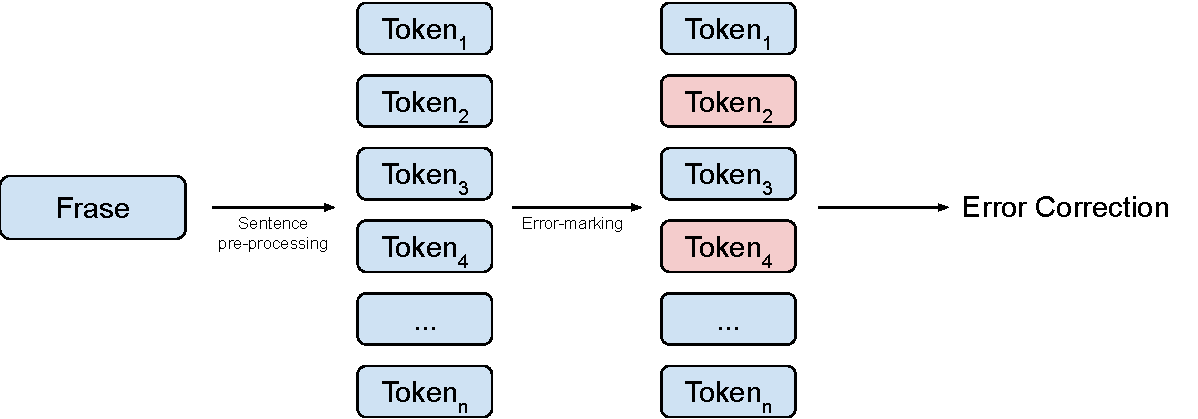
\includegraphics[width=\textwidth]{immagini/metodologia/error_detection}
\caption{Schema del processo di error detection}
\label{fig:met_tok_errdet}
\end{figure}

\subsubsection{Error Correction}
\label{sec:met_errcor}

La fase di error correction ha lo scopo di correggere gli errori individuati nella precedente fase. La fase di error correction è composta dai seguenti stadi:

\begin{enumerate}
\item Mascheramento
\item Detokenizzazione
\item Generazione e scelta dei candidati
\item Validazione
\end{enumerate}

Ognuno di questi stadi è ripetuto per ognuno degli errori identificati durante la fase precedente.

\begin{figure}[H]
\centering
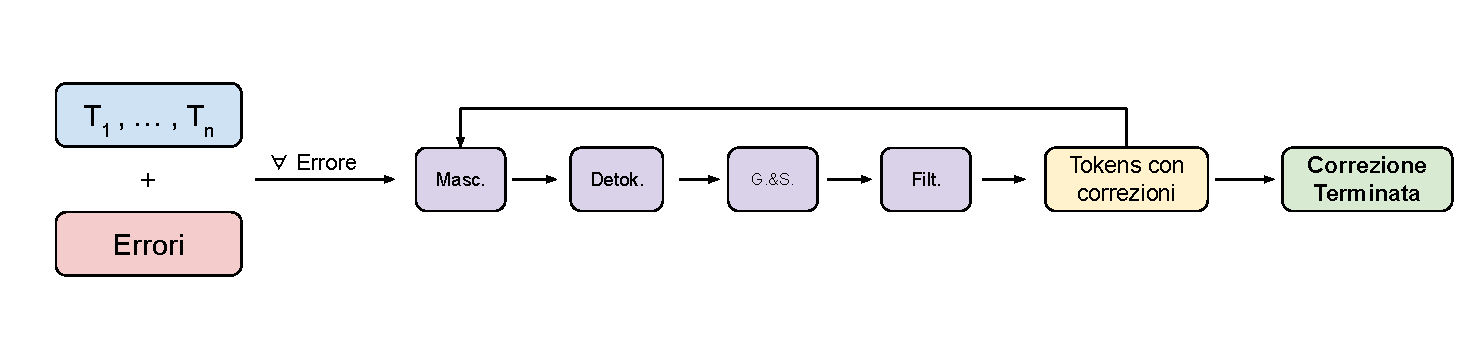
\includegraphics[width=\textwidth]{immagini/metodologia/tok_correction}
\caption{Schema della fase di error correction}
\label{fig:met_tok_correction}
\end{figure}



\paragraph{Mascheramento}
Lo stadio di mascheramento ha lo scopo di mascherare uno dei token errati individuati nella fase precedente. Si ricorda che, a causa del funzionamento del BERT MLM descritto nella \autoref{sec:met_BERT_MLM}, è possibile mascherare solo un token alla volta.\\
Data una sequenza di token $S = [t_1,...,t_n]$ e l'insieme $E = [t_i,t_j,...]\subseteq S$ dei token contenenti errore non ancora corretti, lo stadio di mascheramento è descritto dalla seguente funzione:
\begin{equation}
M: S \rightarrow [t_1,...,\text{[MASK]},...,t_n] = S\prime
\end{equation}
dove \textit{[MASK]} sostituisce il primo token estratto dall'insieme $E$. Quanto descritto corrisponde al primo passaggio nella \autoref{fig:met_errgen}.


\paragraph{Detokenizzazione}
Come spiegato nella \autoref{sec:met_BERT_MLM}, la funzione di mask-filling del BERT MLM richiede come input una sequenza intesa come frase, e non come insieme di token. \E\ quindi compito dello stadio di detokenizzazione ricomporre una sequenza a partire dall'output dello stadio precedente. Lo stadio di detokenizzazione è descritto dalla seguente funzione:
\begin{equation}
D: [t_1,...,\text{[MASK]},...,t_n] \rightarrow F_{mask}
\end{equation}
dove $F_{mask}$ è una frase contente una maschera.

\paragraph{Generazione e scelta dei candidati}
Lo stadio di generazione e scelta dei candidati sfrutta il BERT MLM per generare dei candidati per la correzione, e sfrutta un'euristica per determinare il candidato con la maggior probabilità di essere corretto (da qui in poi riferito come soluzione). Più precisamente, la generazione dei candidati avviene tramite la funzione di mask-filling descritta nell'\autoref{eq:met_BERT} (\autoref{sec:met_BERT_MLM}). La fattibilità di applicare tale approccio per la generazione di candidati per la correzione è dimostrata in \cite{OCRMaskFilling}. Nel paper appena citato si riporta come, usando una combinazione di BERT e FastText, la giusta correzione da applicare sia presente fra i candidati prodotti con una probabilità del 70\%. \hl{TODO: inserire riferimento ai risultati del capitolo analisi errore.}\\
Lo step di generazione dei candidati è formalizzato come segue:
\begin{equation}
G: F_{mask} \rightarrow [c_1,...,c_n]= C
\end{equation}
dove ogni $c_i$ è un candidato.\\
L'euristica per la scelta della soluzione sceglie il candidato con la più bassa distanza di Levenshtein dal token mascherato. Più formalmente, chiamando $m$ il token mascherato, la soluzione $s$ è definita come segue:
\begin{equation}
s = \operatorname*{argmin}_{c_i \in C} d_{lev}(c_i,m)
\end{equation}
In caso uno o più candidati abbiamo la stessa distanza dal token mascherato, viene scelto quello con la maggior probabilità prodotta da BERT.
\hl{TODO: giustificazione dell'euristica attraverso risultato presenti nel capitolo di analisi errore}

\begin{figure}[H]
\centering
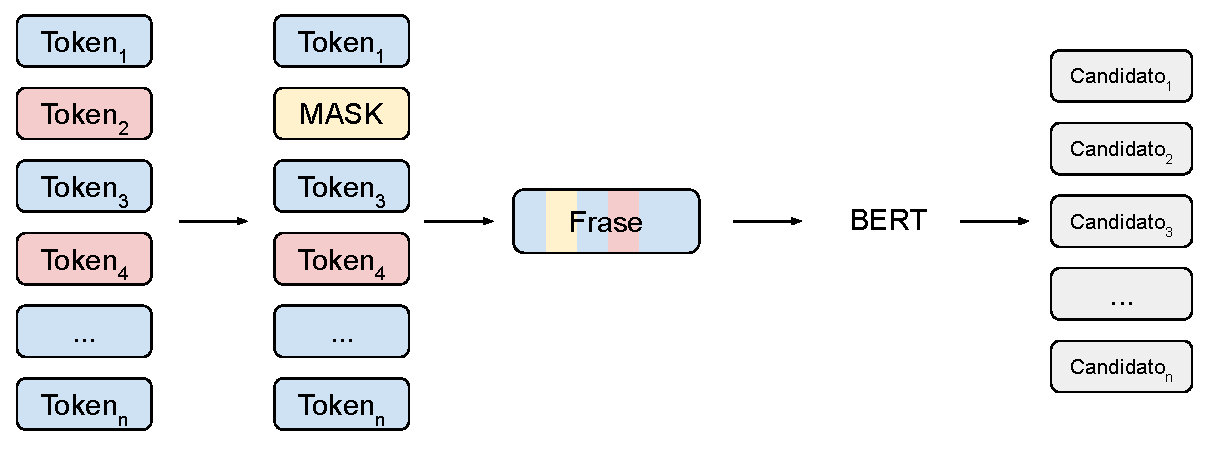
\includegraphics[width=\textwidth]{immagini/metodologia/generazione_candidati}
\caption{Schema del processo di generazione e scelta dei candidati}
\label{fig:met_errgen}
\end{figure}

\paragraph{Validazione}
Può accadere che la soluzione non sia una correzione adatta: si pensi ai seguenti casi:
\begin{enumerate}
\item L'error detection contrassegna un token corretto come errore. In questo caso, ogni tentativo di correzione introdurrebbe nuovi errori all'interno del testo.
\item BERT non produce la giusta correzione fra i candidati. Anche in questo caso, qualunque sia il candidato scelto, il sistema di correzione andrebbe a introdurre nuovi errori all'interno del testo.
\end{enumerate}

\E\ introdotta quindi un'ulteriore fase di validazione, con lo scopo di valutare se la soluzione prodotta possa o meno rappresentare una correzione valida. La validazione è implementata tramite un'euristica che valuta se la soluzione trovata è troppo lontana (in termini di distanza di Levenshtein) dal token mascherato. Chiamando $l$ la lunghezza in caratteri del token mascherato, e $d$ la distanza di Levenshtein fra il token mascherato e la soluzione trovata, la soluzione è valida se:
\begin{itemize}
\item $l > 10 \wedge d < 5$ 
\item $l > 5 \wedge d < 4$ 
\item $l \leqslant 5 \wedge d < 3$ 
\end{itemize}
Se la validazione scarta la soluzione trovata il sistema ignora la correzione. Al contrario, se la validazione ritorna esito positivo, la correzione viene sostituita al token mascherato. Quanto appena descritto è rappresentato in \autoref{fig:met_pick}.

\begin{figure}[H]
\centering
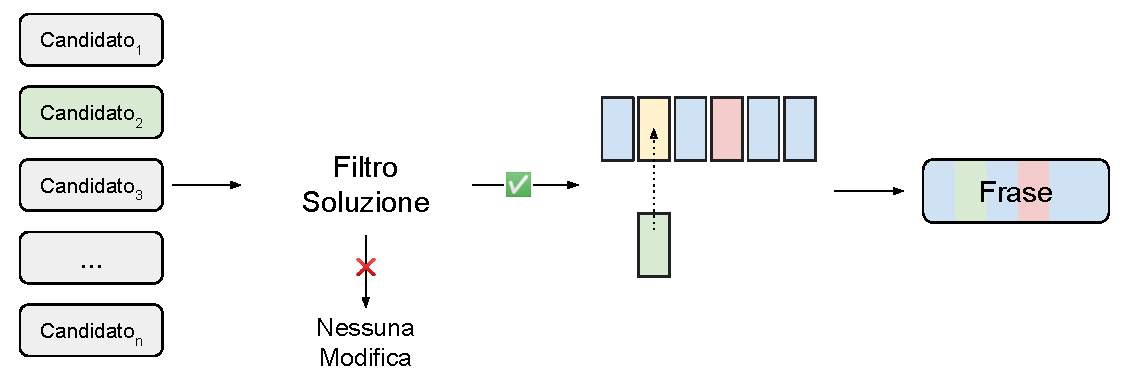
\includegraphics[width=\textwidth]{immagini/metodologia/scelta_candidati}
\caption{Schema del processo di scelta dei candidati}
\label{fig:met_pick}
\end{figure}
Il processo appena descritto si ripete per ogni errore contrassegnato durante la fase di error detection. Una volta completata la correzione dell'ultimo token errato, la fase di error correction può dirsi conclusa.

\subsubsection{Ripetizione}
In frasi contenenti molti errori, è possibile che una sola applicazione del modulo di correzione token non basti correggere tutti i non-word errors. Ciò è dovuto al funzionamento di BERT, che usa il contesto a destra e sinistra della maschera per produrre i candidati di correzione. Se questo contesto è sporcato da molti errori, è più probabile che BERT non sia in grado di produrre una soluzione adeguata. \E\ quindi possibile che dopo l'applicazione di questo o altri moduli, e la conseguente correzione di alcuni errori, sia possibile ottenere migliori risultati sulle correzioni precedentemente non riuscite.

\subsection{Modulo di correzione Split}
\label{sec:met_mod_split}

\subsubsection{Error detection}
\label{sec:met_split_errdet}
Il modulo di correzione Split corregge tutti gli errori di spezzettamento con spazi (SP).
La fase di error detection si compone di tre stadi:
\begin{enumerate}
\item \textbf{Individuazione delle sequenze}: data un frase contenente errori di tipo SP, sono delimitati i punti di inizio e terminazione delle sequenze contenenti errori. L'individuazione di tali sequenze è eseguita tramite la seguente espressione regolare:
\begin{lstlisting}[language=Python]
r'(?:\s|^)(\w(?:\W?\s\w{1,2}){3,})(?:\W|\s|$)'
\end{lstlisting}
La precedente espressione regolare intercetta tutte le sequenze di almeno tre gruppi di caratteri alfanumerici con lunghezza massima due intervallati da spazi e/o caratteri non alfanumerici. Per maggiore chiarezza, in \autoref{table:met_split_esempi} sono riportati alcuni esempi di sequenze riconosciute.

\item \textbf{Filtraggio punteggiatura}: all'interno delle sequenze vengono rimossi tutti i caratteri non alfanumerici. Ciò serve e rimuovere eventuali segni di punteggiatura spuri che possono diminuire l'efficacia delle seguenti fasi.

\item \textbf{Validazione errore:} non tutte le sequenze riconosciute dall'espressione regolare sono degli errori. Si pensi ad esempio ad una serie di preposizioni o congiunzioni, come il quarto esempio in \autoref{table:met_split_esempi}. Si usa quindi un'euristica per scartare le sequenze che si ritenga non contengano errori. Sono considerati errori tutte le sequenze nelle quali il numero di gruppi di 2 caratteri è minore del numero di gruppi di 1 carattere.

\end{enumerate}


\begin{table}[H]
	\centering
	\begin{tabular}{ccc}
	\textbf{Frase} & \textbf{Sequenza} & \textbf{Errore} \\ \hline
	
	\textit{"d i l e t t i membri, della ..."}	&	\textit{d i l e t t i}	&	Sì \\
	\textit{"guidato d ui l l a fede"}			& 	\textit{d ui l l a}		&	Sì \\
	\textit{"... altro tipo di u n i o, n e."}	&	\textit{u n i o, n e}	&	Sì \\
	\textit{"in me e io in te, siano anch..."}	&	\textit{in me e io in te}&	No
	\end{tabular}
	\caption{Esempi di sequenze riconosciute}
	\label{table:met_split_esempi}
\end{table}

Data quindi una frase $F$ contenente errori di segmentazione, la fase di error detection è formalizzata come segue:
\begin{equation}
\textit{ED}_{split}: F \rightarrow [(s_1,b_1,e_1),...,(s_n,b_n,e_n)]
\end{equation}
dove:
\begin{itemize}
\item Ogni tupla corrisponde ad un errore individuato e validato
\item $s_i$ è la sequenza filtrata contenente l'errore
\item $b_i$ è il punto di inizio in $F$ della sequenza
\item $e_i$ è il punto di fine in $F$ delle sequenze
\end{itemize}

\begin{figure}[H]
\centering
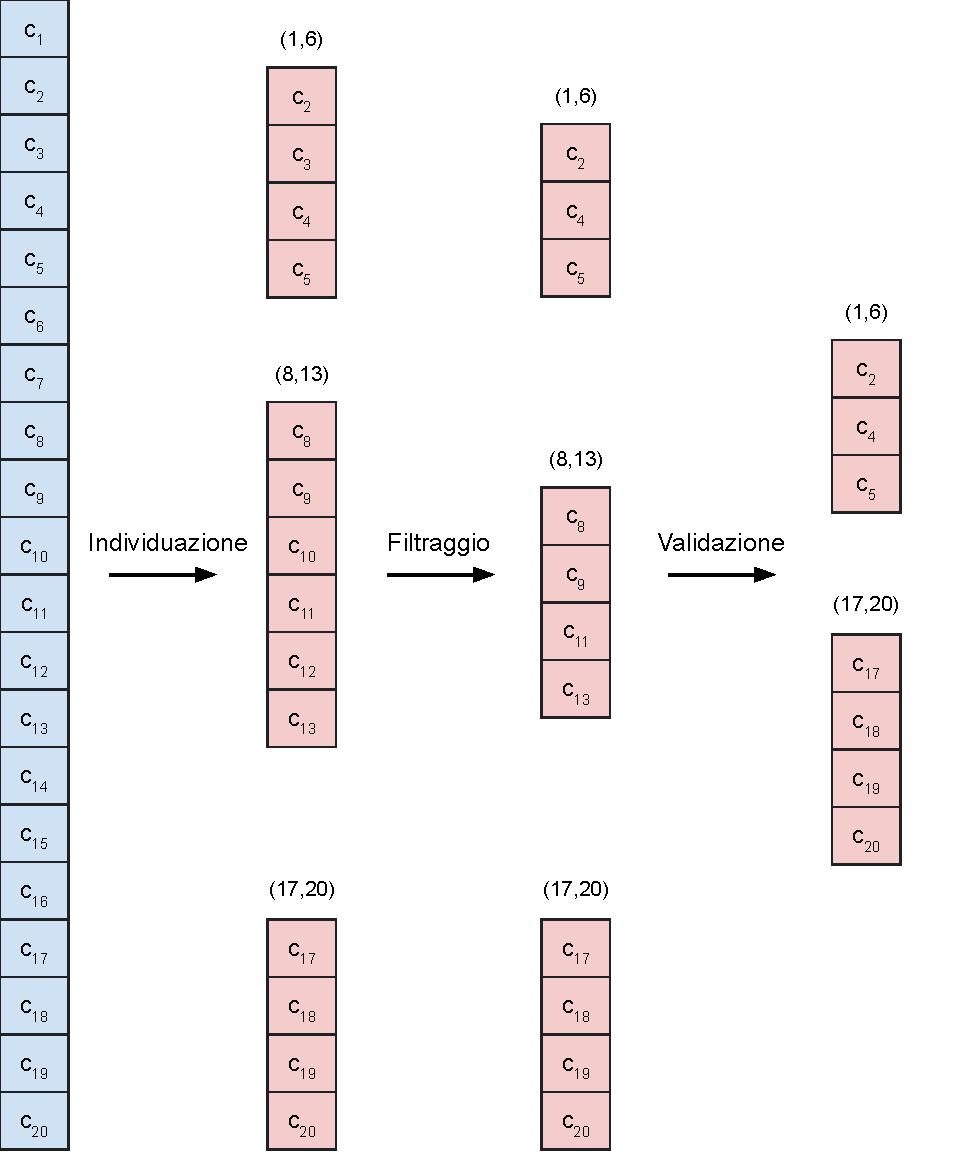
\includegraphics[width=\textwidth]{immagini/metodologia/split_error_detection}
\caption{Schema del processo di error detection. Nell'immagine, ogni $c_i$ è un carattere}
\label{fig:met_split_errdet}
\end{figure}

\paragraph{Esempio}
Data la frase:
\begin{center}
\textit{coinvolsero ogni uomo \ul{e o' g n i} donna, \ul{p r o c u r a n d o}.}
\end{center}
si procede con lo stadio di individuazione delle sequenze. Le sequenze individuate sono quello sottolineate nella frase data. Sono riportate di seguito, nel seguente formato (sequenza,posizione inizio sequenza, posizione fine sequenza):
\begin{enumerate}
\item \textit{"e o' g n i"}, 22, 32
\item \textit{"p r o c u r a n d o"}, 40, 59
\end{enumerate}

Si procede quindi con lo stadio di filtraggio:
\begin{enumerate}
\item \textit{"e o g n i"}, 22, 32
\item \textit{"p r o c u r a n d o"}, 40, 59
\end{enumerate}
Si noti come nella prima sequenza è stato cancellato un apostrofo, ma le posizioni di inizio e fine rimangono le stesse. Lo stadio di validazione in questo caso non scarta alcuna soluzione: in entrambe le sequenze, infatti, il numero di gruppi di 1 carattere è maggiore del numero di gruppi di 2 caratteri.

\subsubsection{Error correction}
\label{sec:met_split_errcor}











